\documentclass[12pt,ngerman,parskip=half]{scrreport}

\usepackage{babel}
\usepackage{blindtext}
\usepackage{graphicx}
\usepackage{booktabs}
\usepackage{xcolor}

\newcommand{\person}[1]{\textcolor{blue}{\textsc{#1}}}

\newcommand{\fuh}{Fernuni Hagen}

\author{Uwe Ziegenhagen}
\title{Mein erstes LaTeX-Dokument}
\date{Köln, den \today} % leerlassen zum Unterdrücken

\begin{document}
\maketitle

\tableofcontents

\listoffigures

\listoftables


\chapter{Einführung}

\section{Einleitung}
% in eckigen Klammern die Kurzversion für's Inhaltsverzeichnis
\subsection[Literaturüberblick über die relevante Literatur]{Literaturüberblick über die relevante Literatur der post-sozialistischen Arbeiterklasse}
\subsubsection{Deutsche Literatur}

Wie wir in Abschnitt \ref{sec:ausblick} sehen werden...

\textcolor{red}{\textsc{Albert Einstein}} und \person{Niels Bohr} waren bedeutende Physiker.

Hallo Fernuni! \fuh\ Ich bin ein einfacher Text.

Um einen neuen Absatz zu beginnen, fügen wir einfach eine Leerzeile ein.

% Formate png, pdf, jpg

% h = here, t = top, b = bottom, p = eigene Seite, !

\begin{figure}[b] % float, htbp!
\begin{center}

\includegraphics[width=10cm]{Bilder/Katze}
\end{center}
\caption{Katze 1}\label{fig:katze}
\end{figure}

\blindtext[1]


\begin{figure}[h]
\begin{center}

\includegraphics[width=0.8\textwidth]{Bilder/miau}
\end{center}
\caption{Katze 2}\label{fig:miau}
\end{figure}

\blindtext[5]


\begin{figure}[b]
\begin{center}
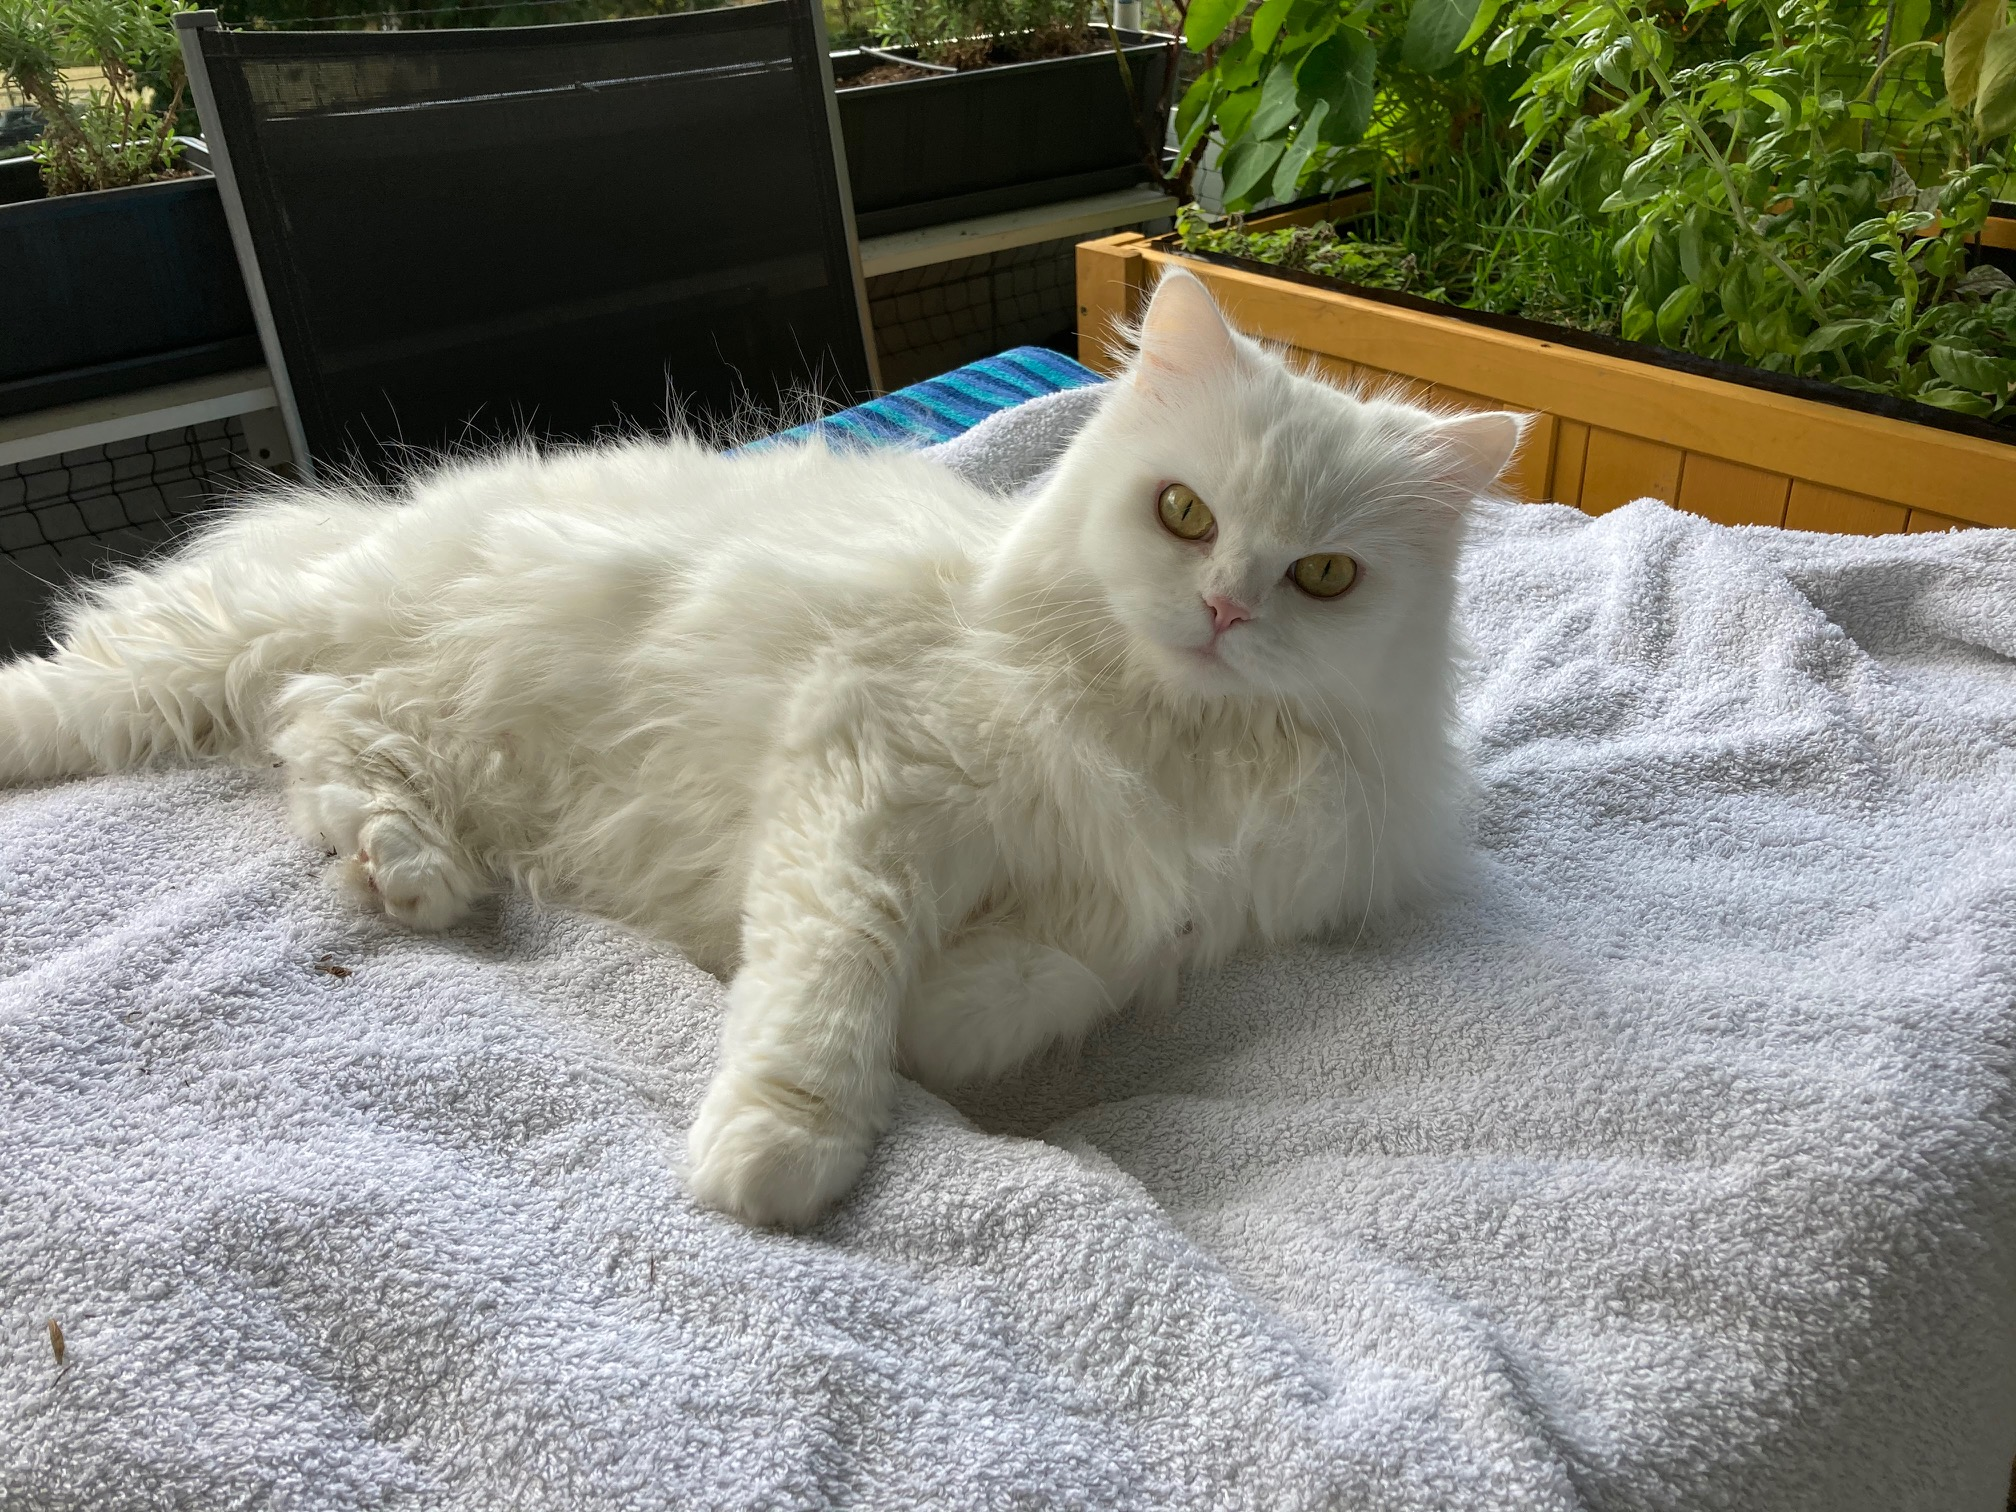
\includegraphics[width=\textwidth]{Bilder/Katze1}
\end{center}
\caption{Katze 3}\label{fig:katze1}
\end{figure}

\blindtext[5]

\section{fdsdfsd}
\subsection{fsdfsdfs}
\subsubsection{Internationale Forschung}

\blindtext

\paragraph{sdfsdf} \blindtext

\subparagraph{sdfsdf} \blindtext


\section{Analyse}

\blindtext[5]

%\pagebreak
\section{Fazit}

\subsection{Ausblick}\label{sec:ausblick} 

Siehe Abbildung \ref{fig:katze} auf Seite \pageref{fig:katze}


\blindtext

\chapter{Tabellen und mehr}

\blindtext

\begin{tabular}{|l|r|c|p{4cm}|} \hline
\textbf{Spalte 1 } & \textbf{Spalte 2}  & \textbf{Spalte 3}  & \textbf{Spalte 4 } \\ \hline
Hallo & ich bwwqe we in &  546464654654 & Hallo, ich bin ein umbrechender Text in einer Tabellenzelle \\
Hallo & ich bin & ein & Text \\
Hallo & ich bin & ein längerer & qweqwqweText \\
Halloqe  eqwe  & ich & sadas asd ad asds da bin & ein Text \\ \hline
\end{tabular}

\begin{tabular}{llll}
Spalte 1	&	Spalte 2	&	Spalte 3	&	Spalte 4	\\
0.54672	&	0.97409	&	0.58197	&	0.76644	\\
0.72276	&	0.50369	&	0.5661	&	0.49698	\\
0.12651	&	0.76127	&	0.17254	&	0.22598	\\
0.28751	&	0.12825	&	0.13667	&	0.92436	\\
0.08554	&	0.39593	&	0.97684	&	0.66707	\\
0.40292	&	0.06858	&	0.41431	&	0.91665	\\
0.43603	&	0.71738	&	0.29055	&	0.13398	\\
0.32662	&	0.65372	&	0.47782	&	0.04812	\\
0.06094	&	0.57221	&	0.3379	&	0.00134	\\
0.44674	&	0.12709	&	0.01823	&	0.5974	\\
0.86293	&	0.69307	&	0.58792	&	0.24032	\\
0.59019	&	0.1569	&	0.78805	&	0.78216	\\
0.63636	&	0.45639	&	0.87984	&	0.57814	\\
0.2254	&	0.67795	&	0.00258	&	0.26288	\\
0.98004	&	0.14941	&	0.53561	&	0.35265	\\
0.37031	&	0.66397	&	0.85259	&	0.0084	\\
0.66199	&	0.30483	&	0.76343	&	0.26389	\\
0.95394	&	0.85443	&	0.44793	&	0.05723	\\
0.1107	&	0.31182	&	0.02327	&	0.64285	\\
0.1956	&	0.30439	&	0.66969	&	0.86096	\\
0.35771	&	0.92456	&	0.09504	&	0.57612	\\
0.0523	&	0.55779	&	0.32854	&	0.54633	\\
0.87916	&	0.06719	&	0.97401	&	0.6816	\\
0.38648	&	0.40777	&	0.43882	&	0.69333	\\
0.55161	&	0.42466	&	0.65779	&	0.78344	\\
\end{tabular}

\begin{table}
\caption{Hallihallo}
\begin{center}
\begin{tabular}{llll} \toprule[2pt]
\addlinespace[0.25cm] \textbf{Spalte 1}	&	\textbf{Spalte 2}	&	\textbf{Spalte 3}	&	\textbf{Spalte 4}	\\ \midrule[1.5pt]
0.54672	&	0.97409	&	0.58197	&	0.76644	\\
0.72276	&	0.50369	&	0.5661	&	0.49698	\\
0.12651	&	0.76127	&	0.17254	&	0.22598	\\
0.28751	&	0.12825	&	0.13667	&	0.92436	\\
0.08554	&	0.39593	&	0.97684	&	0.66707	\\
0.40292	&	0.06858	&	0.41431	&	0.91665	\\
0.43603	&	0.71738	&	0.29055	&	0.13398	\\
0.32662	&	0.65372	&	0.47782	&	0.04812	\\
0.06094	&	0.57221	&	0.3379	&	0.00134	\\
0.44674	&	0.12709	&	0.01823	&	0.5974	\\
0.86293	&	0.69307	&	0.58792	&	0.24032	\\
0.59019	&	0.1569	&	0.78805	&	0.78216	\\
0.63636	&	0.45639	&	0.87984	&	0.57814	\\
0.2254	&	0.67795	&	0.00258	&	0.26288	\\
0.98004	&	0.14941	&	0.53561	&	0.35265	\\
0.37031	&	0.66397	&	0.85259	&	0.0084	\\
0.66199	&	0.30483	&	0.76343	&	0.26389	\\
0.95394	&	0.85443	&	0.44793	&	0.05723	\\
0.1107	&	0.31182	&	0.02327	&	0.64285	\\
0.1956	&	0.30439	&	0.66969	&	0.86096	\\
0.35771	&	0.92456	&	0.09504	&	0.57612	\\
0.0523	&	0.55779	&	0.32854	&	0.54633	\\
0.87916	&	0.06719	&	0.97401	&	0.6816	\\
0.38648	&	0.40777	&	0.43882	&	0.69333	\\
0.55161	&	0.42466	&	0.65779	&	0.78344	\\ \bottomrule[2pt]
\end{tabular}
\end{center}
\end{table}

\textbf{fettgedruckt} % boldface

\textit{kursiv} % italic

\textsl{geneigt} % slanted

\textbf{\textit{fettkursiv}}

\textsc{Kapitälchen} % small caps


\begin{itemize}
\item Hallo
\item ich
\item bin
\item eine Aufzählung
\end{itemize}


\begin{enumerate}
\item Hallo
\item ich
\item bin
\item eine Aufzählung
\end{enumerate}

\begin{description}
\item [Äpfel] Hallo
\item [b] ich
\item [Birne] bin
\item [d] eine Aufzählung
\end{description}

\begin{itemize}
\item Hallo
\item ich 

\begin{itemize}
\item Hallo
\item ich
\item bin

\begin{itemize}
\item Hallo
\item ich
\item bin
\item eine Aufzählung
\end{itemize}

\item eine Aufzählung
\end{itemize}


\item bin
\item eine Aufzählung
\end{itemize}


\end{document}




